% Seminar 3: Modele ARIMA
% Prezentare academică de calitate Harvard
% Program de licență, Academia de Studii Economice din București

\documentclass[9pt, aspectratio=169, t]{beamer}

% Asigură încadrarea conținutului pe diapozitive
\setbeamersize{text margin left=8mm, text margin right=8mm}

%=============================================================================
% CONFIGURARE TEMĂ ȘI STIL
%=============================================================================
\usetheme{default}

% Color Palette (matching Redispatch PDF)
\definecolor{MainBlue}{RGB}{26, 58, 110}
\definecolor{AccentBlue}{RGB}{26, 58, 110}
\definecolor{IDAred}{RGB}{205, 0, 0}
\definecolor{DarkGray}{RGB}{51, 51, 51}
\definecolor{MediumGray}{RGB}{128, 128, 128}
\definecolor{LightGray}{RGB}{248, 248, 248}
\definecolor{VeryLightGray}{RGB}{235, 235, 235}
\definecolor{KeynoteGray}{RGB}{218, 218, 218}
\definecolor{SectionGray}{RGB}{120, 120, 120}
\definecolor{FooterGray}{RGB}{100, 100, 100}
\definecolor{Crimson}{RGB}{220, 53, 69}
\definecolor{Forest}{RGB}{46, 125, 50}
\definecolor{Amber}{RGB}{181, 133, 63}
\definecolor{Orange}{RGB}{230, 126, 34}
\definecolor{Purple}{RGB}{142, 68, 173}

% Gradient background (exact Keynote 315 gradient: white to RGB 218,218,218)
\setbeamertemplate{background}{%
    \begin{tikzpicture}[remember picture, overlay]
        \shade[shading=axis, shading angle=315,
        top color=white, bottom color=KeynoteGray]
        (current page.south west) rectangle (current page.north east);
    \end{tikzpicture}%
}
% Fallback solid color for compatibility
\setbeamercolor{background canvas}{bg=}

\setbeamercolor{palette primary}{bg=MainBlue, fg=white}
\setbeamercolor{palette secondary}{bg=MainBlue!85, fg=white}
\setbeamercolor{palette tertiary}{bg=MainBlue!70, fg=white}
\setbeamercolor{structure}{fg=MainBlue}
\setbeamercolor{title}{fg=IDAred}
\setbeamercolor{frametitle}{fg=IDAred, bg=}
\setbeamercolor{block title}{bg=MainBlue, fg=white}
\setbeamercolor{block body}{bg=VeryLightGray, fg=DarkGray}
\setbeamercolor{block title alerted}{bg=Crimson, fg=white}
\setbeamercolor{block body alerted}{bg=Crimson!8, fg=DarkGray}
\setbeamercolor{block title example}{bg=Forest, fg=white}
\setbeamercolor{block body example}{bg=Forest!8, fg=DarkGray}
\setbeamercolor{item}{fg=MainBlue}

% Footer colors (override Madrid theme blue)
\setbeamercolor{author in head/foot}{fg=FooterGray, bg=}
\setbeamercolor{title in head/foot}{fg=FooterGray, bg=}
\setbeamercolor{date in head/foot}{fg=FooterGray, bg=}
\setbeamercolor{section in head/foot}{fg=FooterGray, bg=}
\setbeamercolor{subsection in head/foot}{fg=FooterGray, bg=}

% Bullet styles (apply everywhere including blocks)
\setbeamertemplate{itemize item}{\color{MainBlue}$\boxdot$}
\setbeamertemplate{itemize subitem}{\color{MainBlue}$\blacktriangleright$}
\setbeamertemplate{itemize subsubitem}{\color{MainBlue}\tiny$\bullet$}
\setbeamertemplate{itemize/enumerate body begin}{\normalsize}
\setbeamertemplate{itemize/enumerate subbody begin}{\normalsize}

% Item spacing - compact style
\setlength{\leftmargini}{10pt}       % Level 1: minimal indent
\setlength{\leftmarginii}{10pt}      % Level 2: minimal additional indent
% Compact list spacing (zero extra space before/after lists in blocks)
\makeatletter
\def\@listi{\leftmargin\leftmargini \topsep 0pt \parsep 0pt \itemsep 0pt}
\def\@listii{\leftmargin\leftmarginii \topsep 0pt \parsep 0pt \itemsep 0pt}
\makeatother

\setbeamertemplate{navigation symbols}{}

%=============================================================================
% CUSTOM HEADLINE
%=============================================================================
\setbeamertemplate{headline}{%
    \vskip10pt%
    \hbox to \paperwidth{%
        \hskip0.5cm%
        {\small\color{FooterGray}\renewcommand{\hyperlink}[2]{##2}\insertsectionhead}%
        \hfill%
        \textcolor{FooterGray}{\small\insertframenumber}%
        \hskip0.5cm%
    }%
    \vskip4pt%
    {\color{FooterGray}\hrule height 0.4pt}%
}

%=============================================================================
% CUSTOM FOOTER
%=============================================================================
\usepackage{fontawesome5}

\setbeamertemplate{footline}{%
    {\color{FooterGray}\hrule height 0.4pt}%
    \vskip4pt%
    \hbox to \paperwidth{%
        \hskip0.5cm%
        \textcolor{FooterGray}{\small Analiza și Prognoza seriilor de timp}%
        \hfill%
        \raisebox{-0.1em}{%
            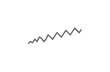
\begin{tikzpicture}[x=0.08em, y=0.08em, line width=0.4pt]
                \draw[FooterGray] (0,3) -- (1,4) -- (2,3.5) -- (3,5) -- (4,4) -- (5,6) -- (6,5.5) -- (7,4) -- (8,5) -- (9,7) -- (10,6) -- (11,5) -- (12,6.5) -- (13,8) -- (14,7) -- (15,6) -- (16,7.5) -- (17,9) -- (18,8) -- (19,7) -- (20,8.5) -- (21,10) -- (22,9) -- (23,8) -- (24,9.5);
            \end{tikzpicture}%
        }%
        \hskip0.5cm%
    }%
    \vskip6pt%
}

%=============================================================================
% PACHETE
%=============================================================================
\usepackage[utf8]{inputenc}
\usepackage[T1]{fontenc}
\usepackage[romanian]{babel}
\usepackage{amsmath, amssymb, amsthm}
\usepackage{mathtools}
\usepackage{bm}
\usepackage{tikz}
\usetikzlibrary{arrows.meta, positioning, shapes, calc, decorations.pathreplacing, shadings}
\usepackage{booktabs}
\usepackage{multirow}
\usepackage{array}
\usepackage{graphicx}
\usepackage{hyperref}
\usepackage{colortbl}
\hypersetup{colorlinks=true, linkcolor=MainBlue, urlcolor=MainBlue}
\graphicspath{{../../logos/}{../../charts/}}
\hfuzz=2pt  % Suppress tiny overfull warnings (<2pt)
\vfuzz=2pt  % Suppress tiny vertical overfull warnings (<2pt)

%=============================================================================
% COMANDA QUANTLET
%=============================================================================
\newcommand{\quantlet}[2]{%
    \hfill\href{#2}{%
        \raisebox{-0.15em}{\includegraphics[height=0.7em]{ql_logo.png}}%
        \textcolor{MainBlue}{\tiny\ #1}%
    }%
}

%=============================================================================
% MEDII PENTRU TEOREME
%=============================================================================
\theoremstyle{definition}
\setbeamertemplate{theorems}[numbered]
\newtheorem{defn}{Definiție}
\newtheorem{thm}{Teoremă}
\newtheorem{prop}{Propoziție}
\newtheorem{rmk}{Observație}

%=============================================================================
%=============================================================================
% CENTRED MINIPAGE (fara spatiu vertical suplimentar)
%=============================================================================
\newenvironment{cminipage}[1]{%
    \par\noindent\hfill\begin{minipage}{#1}\ignorespaces
}{%
    \end{minipage}\hfill\null\par
}


% COMENZI PERSONALIZATE
%=============================================================================
\newcommand{\E}{\mathbb{E}}
\newcommand{\Var}{\text{Var}}
\newcommand{\Cov}{\text{Cov}}
\newcommand{\Corr}{\text{Corr}}
\newcommand{\R}{\mathbb{R}}
\newcommand{\N}{\mathbb{N}}
\newcommand{\Z}{\mathbb{Z}}
\newcommand{\RMSE}{\text{RMSE}}
\newcommand{\MAE}{\text{MAE}}
\newcommand{\MAPE}{\text{MAPE}}

\newcommand{\correct}{\textcolor{Forest}{\checkmark}}
\newcommand{\incorrect}{\textcolor{Crimson}{\texttimes}}

%=============================================================================
% PAGINĂ TITLU PERSONALIZATĂ
%=============================================================================
\defbeamertemplate*{title page}{hybrid}[1][]
{
    \vspace{0.2cm}
    \begin{center}
        \href{https://www.ase.ro}{\includegraphics[height=1.0cm]{ase_logo.png}}\hspace{0.3cm}%
        \href{https://theida.net}{\includegraphics[height=1.0cm]{ida_logo.png}}\hspace{0.3cm}%
        \href{https://blockchain-research-center.com}{\includegraphics[height=1.0cm]{brc_logo.png}}\hspace{0.3cm}%
        \href{https://www.ai4efin.ase.ro}{\includegraphics[height=1.0cm]{ai4efin_logo.png}}\hspace{0.3cm}%
        \href{https://ipe.ro/new}{\includegraphics[height=1.0cm]{acad_logo.png}}\hspace{0.3cm}%
        \href{https://www.digital-finance-msca.com}{\includegraphics[height=1.0cm]{msca_logo.png}}%
    \end{center}

    \vspace{0.6cm}

    \begin{center}
        \begin{minipage}{0.1\textwidth}
            \centering
            \href{https://quantlet.com}{\includegraphics[height=1.1cm]{ql_logo.png}}
        \end{minipage}%
        \begin{minipage}{0.78\textwidth}
            \centering
            {\LARGE\bfseries\usebeamercolor[fg]{title}\inserttitle}

            \vspace{0.3cm}

            {\usebeamerfont{subtitle}\usebeamercolor[fg]{title}\insertsubtitle}
        \end{minipage}%
        \begin{minipage}{0.1\textwidth}
            \centering
            \href{https://quantinar.com}{\includegraphics[height=1.1cm]{qr_logo.png}}
        \end{minipage}
    \end{center}

    \vspace{0.6cm}

    \hspace{0.5cm}{\usebeamerfont{author}\insertauthor}

    \vspace{0.3cm}

    \hspace{0.5cm}\begin{minipage}[t]{0.9\textwidth}
        \raggedright\small\insertinstitute
    \end{minipage}
}

%=============================================================================
% INFORMAȚII TITLU
%=============================================================================
\title[Analiza Seriilor de Timp]{Analiza și Prognoza seriilor de timp}
\subtitle{Seminar 3: Modele ARIMA}
\author[D.T. Pele]{Daniel Traian PELE}
\institute{Academia de Studii Economice din București\\
IDA Institute Digital Assets\\
Blockchain Research Center\\
AI4EFin Artificial Intelligence for Energy Finance\\
Academia Română, Institutul de Prognoză Economică\\
MSCA Digital Finance}
\date{}

\begin{document}

% Title page (no header/footer)
{
\setbeamertemplate{headline}{}
\setbeamertemplate{footline}{}
\begin{frame}
    \titlepage
\end{frame}
}

%=============================================================================
% PREZENTARE GENERALĂ
%=============================================================================
\section{Prezentare Generală}

\begin{frame}{Cuprins Seminar}
    \begin{cminipage}{0.95\textwidth}
    \textbf{\large Activitățile de Astăzi:}

    \vspace{0.4cm}

    \begin{enumerate}
        \item[\textcolor{MainBlue}{\textbf{1.}}] \textbf{Test de Recapitulare} --- Verificarea înțelegerii conceptelor ARIMA
        \vspace{0.15cm}
        \item[\textcolor{MainBlue}{\textbf{2.}}] \textbf{Întrebări Adevărat/Fals} --- Verificări conceptuale
        \vspace{0.15cm}
        \item[\textcolor{MainBlue}{\textbf{3.}}] \textbf{Probleme Practice} --- Calcule cu ARIMA
        \vspace{0.15cm}
        \item[\textcolor{MainBlue}{\textbf{4.}}] \textbf{Exemple Rezolvate} --- Aplicații din lumea reală
        \vspace{0.15cm}
        \item[\textcolor{MainBlue}{\textbf{5.}}] \textbf{Analiză pe Date Reale} --- Studiu de caz PIB
        \vspace{0.15cm}
        \item[\textcolor{MainBlue}{\textbf{6.}}] \textbf{Exerciții AI} --- Modelare om vs.\ AI
    \end{enumerate}
    \end{cminipage}
\end{frame}

%=============================================================================
% SECTION 1: REVIEW QUIZ
%=============================================================================
\section{Test de Recapitulare}

\begin{frame}{Test 1: Ordinul de Integrare}
    \begin{cminipage}{0.95\textwidth}
    \begin{alertblock}{Întrebare}
        O serie de timp $Y_t$ necesită două diferențe pentru a deveni staționară. Care este ordinul ei de integrare?
    \end{alertblock}
    \vspace{0.1cm}

    \only<1>{
    \begin{block}{Variante de răspuns}
        \textcolor{MainBlue}{\textbf{(A)}} $I(0)$ \qquad
{indent}    \textcolor{MainBlue}{\textbf{(B)}} $I(1)$ \qquad
{indent}    \textcolor{MainBlue}{\textbf{(C)}} $I(2)$ \qquad
{indent}    \textcolor{MainBlue}{\textbf{(D)}} Nu poate fi determinat
    \end{block}
    }
    \only<2>{
    \begin{exampleblock}{Răspuns: C -- $I(2)$}
        \textbf{Definiție}: $Y_t \sim I(d)$ dacă $\Delta^d Y_t$ este staționară dar $\Delta^{d-1} Y_t$ nu este.

        \textbf{Exemplu}: Dacă $Y_t$ urmează $\Delta^2 Y_t = \varepsilon_t$, atunci:
        \begin{itemize}
            \item $\Delta Y_t = \Delta Y_{t-1} + \varepsilon_t$ (încă are rădăcină unitară)
            \item $\Delta^2 Y_t = \varepsilon_t$ (zgomot alb, staționară)
        \end{itemize}

        \textbf{Lumea reală}: Indicii de prețuri pot fi $I(2)$ când inflația însăși este nestaționară.
    \end{exampleblock}
    }
    \end{cminipage}
\end{frame}

\begin{frame}{Vizual: Procese Integrate}
    \begin{cminipage}{0.95\textwidth}
    \begin{center}
        \includegraphics[width=0.90\textwidth, height=0.65\textheight, keepaspectratio]{ch3_def_integrated.pdf}
    \end{center}
    \vspace{-0.3cm}
    {\footnotesize $I(0)$: staționară. $I(1)$: o diferență necesară. $I(2)$: două diferențe necesare pentru a deveni staționară.}

    \end{cminipage}
    \quantlet{TSA\_ch3\_def\_integrated}{https://github.com/QuantLet/TSA/tree/main/TSA_ch3/TSA_ch3_differencing}
\end{frame}

\begin{frame}{Test 2: Proprietățile Mersului Aleatoriu}
    \begin{cminipage}{0.95\textwidth}
    \begin{alertblock}{Întrebare}
        Pentru un mers aleator $Y_t = Y_{t-1} + \varepsilon_t$ cu $\Var(\varepsilon_t) = \sigma^2$, care este $\Var(Y_t)$?
    \end{alertblock}
    \vspace{0.3cm}
    \begin{center}
        \includegraphics[width=0.75\textwidth, height=0.38\textheight, keepaspectratio]{sem3_rw_variance.pdf}
    \end{center}

    \end{cminipage}
    \quantlet{TSA\_ch3\_rw\_variance}{https://github.com/QuantLet/TSA/tree/main/TSA_ch3/TSA_ch3_variance_growth}
\end{frame}

\begin{frame}{Test 3: Ipotezele Testului ADF}
    \begin{cminipage}{0.95\textwidth}
    \begin{alertblock}{Întrebare}
        În testul Augmented Dickey-Fuller, care este ipoteza nulă?
    \end{alertblock}
    \vspace{0.1cm}

    \only<1>{
    \begin{block}{Variante de răspuns}
        \textcolor{MainBlue}{\textbf{(A)}} Seria este staționară \qquad
{indent}    \textcolor{MainBlue}{\textbf{(B)}} Seria are o rădăcină unitară \qquad
{indent}    \textcolor{MainBlue}{\textbf{(C)}} Seria nu are autocorelație \qquad
{indent}    \textcolor{MainBlue}{\textbf{(D)}} Seria este distribuită normal
    \end{block}
    }
    \only<2>{
    \begin{exampleblock}{Răspuns: B -- Seria are o rădăcină unitară}
        \textbf{Regresia ADF}: $\Delta Y_t = \alpha + \gamma Y_{t-1} + \sum_{j=1}^{p}\delta_j \Delta Y_{t-j} + \varepsilon_t$

        \textbf{Ipoteze}:
        \begin{itemize}
            \item $H_0: \gamma = 0$ (rădăcină unitară, nestaționară)
            \item $H_1: \gamma < 0$ (staționară)
        \end{itemize}

        \textbf{Decizie}: Respingem $H_0$ dacă statistica $t <$ valoarea critică (de ex., $-2.86$ la 5\%)

        \textbf{Notă}: Folosește distribuția specială Dickey-Fuller, nu $t$ standard.
    \end{exampleblock}
    }
    \end{cminipage}
\end{frame}

\begin{frame}{Vizual: Testul ADF}
    \begin{cminipage}{0.95\textwidth}
    \begin{center}
        \includegraphics[width=0.95\textwidth]{ch3_def_adf.pdf}
    \end{center}
    \vspace{-0.2cm}
    \small Stânga: staționară -- ADF respinge rădăcina unitară. Dreapta: nestaționară -- ADF nu respinge.
    \quantlet{TSA\_ch3\_def\_adf}{https://github.com/QuantLet/TSA/tree/main/TSA_ch3/TSA_ch3_adf_test}
    \end{cminipage}
\end{frame}

\begin{frame}{Test 4: Notația ARIMA}
    \begin{cminipage}{0.95\textwidth}
    \begin{alertblock}{Întrebare}
        Ce înseamnă ARIMA(2,1,1)?
    \end{alertblock}
    \vspace{0.1cm}

    \only<1>{
    \begin{block}{Variante de răspuns}
        \textcolor{MainBlue}{\textbf{(A)}} AR(2) pe date diferențiate cu erori MA(1)\\[3pt]
        \textcolor{MainBlue}{\textbf{(B)}} AR(1) cu 2 diferențe și MA(1)\\[3pt]
        \textcolor{MainBlue}{\textbf{(C)}} MA(2) cu 1 diferență și AR(1)\\[3pt]
        \textcolor{MainBlue}{\textbf{(D)}} 2 lag-uri, 1 trend, 1 componentă sezonieră
    \end{block}
    }
    \only<2>{
    \begin{exampleblock}{Răspuns: A -- AR(2) pe date diferențiate cu erori MA(1)}
        \textbf{ARIMA($p,d,q$)}: $\phi(L)(1-L)^d Y_t = \theta(L)\varepsilon_t$

        \textbf{ARIMA(2,1,1) se expandează la}:
        \[
        (1-\phi_1 L - \phi_2 L^2)(1-L)Y_t = (1+\theta_1 L)\varepsilon_t
        \]
        Sau echivalent: $(1-\phi_1 L - \phi_2 L^2)\Delta Y_t = (1+\theta_1 L)\varepsilon_t$

        \textbf{Interpretare}: Mai întâi diferențiem seria, apoi ajustăm ARMA(2,1) pe $\Delta Y_t$.
    \end{exampleblock}
    }
    \end{cminipage}
\end{frame}

\begin{frame}{Vizual: Procesul ARIMA}
    \begin{cminipage}{0.95\textwidth}
    \begin{center}
        \includegraphics[width=0.90\textwidth, height=0.65\textheight, keepaspectratio]{ch3_def_arima.pdf}
    \end{center}
    \vspace{-0.3cm}
    {\footnotesize Sus: seria ARIMA originală. Jos: după diferențiere, folosim ACF/PACF pentru a identifica ordinele AR și MA.}

    \end{cminipage}
    \quantlet{TSA\_ch3\_def\_arima}{https://github.com/QuantLet/TSA/tree/main/TSA_ch3/TSA_ch3_arima_model}
\end{frame}

\begin{frame}{Test 5: Operatorul de Diferență}
    \begin{cminipage}{0.95\textwidth}
    \begin{alertblock}{Întrebare}
        Care este $(1-L)^2 Y_t$ expandat?
    \end{alertblock}
    \vspace{0.1cm}

    \only<1>{
    \begin{block}{Variante de răspuns}
        \textcolor{MainBlue}{\textbf{(A)}} $Y_t - Y_{t-1}$ \qquad
{indent}    \textcolor{MainBlue}{\textbf{(B)}} $Y_t - 2Y_{t-1} + Y_{t-2}$ \qquad
{indent}    \textcolor{MainBlue}{\textbf{(C)}} $Y_t + 2Y_{t-1} + Y_{t-2}$ \qquad
{indent}    \textcolor{MainBlue}{\textbf{(D)}} $Y_t - Y_{t-2}$
    \end{block}
    }
    \only<2>{
    \begin{exampleblock}{Răspuns: B -- $Y_t - 2Y_{t-1} + Y_{t-2}$}
        \textbf{Expandare folosind teorema binomială}:
        \[
        (1-L)^2 = 1 - 2L + L^2
        \]
        \textbf{Aplicare lui $Y_t$}:
        \[
        (1-L)^2 Y_t = Y_t - 2L \cdot Y_t + L^2 \cdot Y_t = Y_t - 2Y_{t-1} + Y_{t-2}
        \]

        \textbf{Notă}: Aceasta este egală cu $\Delta(\Delta Y_t) = \Delta Y_t - \Delta Y_{t-1}$, ``schimbarea schimbărilor''.
    \end{exampleblock}
    }
    \end{cminipage}
\end{frame}

\begin{frame}{Test 6: KPSS vs ADF}
    \begin{cminipage}{0.95\textwidth}
    \begin{alertblock}{Întrebare}
        Cum diferă testul KPSS de testul ADF?
    \end{alertblock}
    \vspace{0.1cm}

    \only<1>{
    \begin{block}{Variante de răspuns}
        \textcolor{MainBlue}{\textbf{(A)}} KPSS testează sezonalitatea, ADF testează trenduri\\[3pt]
        \textcolor{MainBlue}{\textbf{(B)}} KPSS are staționaritatea ca nulă, ADF are rădăcina unitară ca nulă\\[3pt]
        \textcolor{MainBlue}{\textbf{(C)}} KPSS este mai puternic decât ADF\\[3pt]
        \textcolor{MainBlue}{\textbf{(D)}} Nu există diferență
    \end{block}
    }
    \only<2>{
    \begin{exampleblock}{Răspuns: B -- Ipoteze nule inversate}
        \vspace{-0.2cm}
        \begin{center}
            \includegraphics[width=0.85\textwidth, height=0.36\textheight, keepaspectratio]{sem3_adf_kpss.pdf}
        \end{center}
        \vspace{-0.2cm}
        {\footnotesize
        \textbf{Strategie}: Folosiți ambele teste împreună pentru inferență robustă!
        }
    \end{exampleblock}
    }

    \end{cminipage}
    \quantlet{TSA\_ch3\_adf\_kpss}{https://github.com/QuantLet/TSA/tree/main/TSA_ch3/TSA_ch3_adf_test}
\end{frame}

\begin{frame}{Test 7: Supradiferențierea}
    \begin{cminipage}{0.95\textwidth}
    \begin{alertblock}{Întrebare}
        Dacă $Y_t \sim I(1)$ și calculăm $\Delta^2 Y_t$, ce se întâmplă?
    \end{alertblock}
    \vspace{0.1cm}

    \only<1>{
    \begin{block}{Variante de răspuns}
        \textcolor{MainBlue}{\textbf{(A)}} Obținem o serie staționară mai bună\\[3pt]
        \textcolor{MainBlue}{\textbf{(B)}} Introducem autocorelație negativă artificială\\[3pt]
        \textcolor{MainBlue}{\textbf{(C)}} Varianța scade\\[3pt]
        \textcolor{MainBlue}{\textbf{(D)}} Nu se schimbă nimic
    \end{block}
    }
    \only<2>{
    \begin{exampleblock}{Răspuns: B -- Autocorelație negativă artificială}
        \vspace{-0.2cm}
        \begin{center}
            \includegraphics[width=0.95\textwidth, height=0.36\textheight, keepaspectratio]{sem3_overdifferencing.pdf}
        \end{center}
        \vspace{-0.2cm}
        {\footnotesize
        \textbf{Diagnostic}: ACF la lag 1 $\approx -0.5$ semnalează supradiferențiere. Reduceți $d$ cu 1!
        }
    \end{exampleblock}
    }

    \end{cminipage}
    \quantlet{TSA\_ch3\_overdifferencing}{https://github.com/QuantLet/TSA/tree/main/TSA_ch3/TSA_ch3_differencing}
\end{frame}

\begin{frame}{Test 8: Varianța Prognozei}
    \begin{cminipage}{0.95\textwidth}
    \begin{alertblock}{Întrebare}
        Pentru un model ARIMA(0,1,0) (mers aleator), cum se comportă varianța prognozei când orizontul $h$ crește?
    \end{alertblock}
    \vspace{0.1cm}

    \only<1>{
    \begin{block}{Variante de răspuns}
        \textcolor{MainBlue}{\textbf{(A)}} Rămâne constantă \qquad
{indent}    \textcolor{MainBlue}{\textbf{(B)}} Scade la zero \qquad
{indent}    \textcolor{MainBlue}{\textbf{(C)}} Crește liniar cu $h$ \qquad
{indent}    \textcolor{MainBlue}{\textbf{(D)}} Convergă la o limită finită
    \end{block}
    }
    \only<2>{
    \begin{exampleblock}{Răspuns: C -- Crește liniar cu $h$}
        \textbf{Prognoza mersului aleatoriu}: $\hat{Y}_{T+h|T} = Y_T$ (cea mai bună prognoză este valoarea curentă)

        \textbf{Eroarea de prognoză}: $Y_{T+h} - \hat{Y}_{T+h|T} = \sum_{i=1}^{h} \varepsilon_{T+i}$

        \textbf{Varianță}:
        \[
        \Var(Y_{T+h} - \hat{Y}_{T+h|T}) = h\sigma^2
        \]

        \textbf{IC 95\%}: $Y_T \pm 1.96\sqrt{h}\sigma$ (se lărgește cu $\sqrt{h}$)
    \end{exampleblock}
    }
    \end{cminipage}
\end{frame}

\begin{frame}{Test 9: Puterea Testului de Rădăcină Unitară}
    \begin{cminipage}{0.95\textwidth}
    \begin{alertblock}{Întrebare}
        Testul ADF are putere scăzută când:
    \end{alertblock}
    \vspace{0.1cm}

    \only<1>{
    \begin{block}{Variante de răspuns}
        \textcolor{MainBlue}{\textbf{(A)}} Dimensiunea eșantionului este foarte mare\\[3pt]
        \textcolor{MainBlue}{\textbf{(B)}} Rădăcina adevărată este aproape dar nu egală cu 1\\[3pt]
        \textcolor{MainBlue}{\textbf{(C)}} Seria nu are trend\\[3pt]
        \textcolor{MainBlue}{\textbf{(D)}} Seria este clar staționară
    \end{block}
    }
    \only<2>{
    \begin{exampleblock}{Răspuns: B -- Rădăcina aproape dar nu egală cu 1}
        \textbf{Exemplu}: AR(1) cu $\phi = 0.95$ vs mers aleator ($\phi = 1$)

        \textbf{Problemă}: Ambele au modele ACF similare (descreștere lentă), dar una este staționară!

        \textbf{Putere scăzută înseamnă}: Probabilitate mare de eroare de tip II (eșec în respingerea lui $H_0$ fals)

        \textbf{Soluții}:
        \begin{itemize}
            \item Dimensiuni mai mari ale eșantionului
            \item Testul Phillips-Perron (robust la heteroscedasticitate)
            \item Teste de rădăcină unitară pe paneluri (serii multiple)
        \end{itemize}
    \end{exampleblock}
    }
    \end{cminipage}
\end{frame}

\begin{frame}{Test 10: Selecția modelului ARIMA}
    \begin{cminipage}{0.95\textwidth}
    \begin{alertblock}{Întrebare}
        După o diferențiere, ACF arată un vârf doar la lag 1, și PACF descrește. Modelul potrivit este:
    \end{alertblock}
    \vspace{0.1cm}

    \only<1>{
    \begin{block}{Variante de răspuns}
        \textcolor{MainBlue}{\textbf{(A)}} ARIMA(1,1,0) \qquad
{indent}    \textcolor{MainBlue}{\textbf{(B)}} ARIMA(0,1,1) \qquad
{indent}    \textcolor{MainBlue}{\textbf{(C)}} ARIMA(1,1,1) \qquad
{indent}    \textcolor{MainBlue}{\textbf{(D)}} ARIMA(0,2,1)
    \end{block}
    }
    \only<2>{
    \begin{exampleblock}{Răspuns: B -- ARIMA(0,1,1)}
        \vspace{-0.2cm}
        \begin{center}
            \includegraphics[width=0.95\textwidth, height=0.36\textheight, keepaspectratio]{sem3_arima_flowchart.pdf}
        \end{center}
        \vspace{-0.2cm}
        {\footnotesize
        \textbf{Model}: ACF se anulează la lag 1, PACF descrește $\Rightarrow$ MA(1) pentru seria diferențiată. Model complet: ARIMA(0,1,1) = IMA(1,1)
        }
    \end{exampleblock}
    }

    \end{cminipage}
    \quantlet{TSA\_ch3\_arima\_flowchart}{https://github.com/QuantLet/TSA/tree/main/TSA_ch3/TSA_ch3_arima_model}
\end{frame}

\begin{frame}{Test 11: Staționaritate în Trend vs Staționaritate în Diferențe}
    \begin{cminipage}{0.95\textwidth}
    \begin{alertblock}{Întrebare}
        Un proces staționar în trend devine staționar prin:
    \end{alertblock}
    \vspace{0.1cm}

    \only<1>{
    \begin{block}{Variante de răspuns}
        \textcolor{MainBlue}{\textbf{(A)}} Luarea diferențelor de ordinul întâi\\[3pt]
        \textcolor{MainBlue}{\textbf{(B)}} Eliminarea trendului determinist prin regresie\\[3pt]
        \textcolor{MainBlue}{\textbf{(C)}} Luarea diferențelor de ordinul doi\\[3pt]
        \textcolor{MainBlue}{\textbf{(D)}} Aplicarea ajustării sezoniere
    \end{block}
    }
    \only<2>{
    \begin{exampleblock}{Răspuns: B -- Eliminarea trendului determinist prin regresie}
        \vspace{-0.2cm}
        \begin{center}
            \includegraphics[width=0.95\textwidth, height=0.36\textheight, keepaspectratio]{sem3_trend_vs_diff.pdf}
        \end{center}
        \vspace{-0.2cm}
        {\footnotesize
        \textbf{Staționar în trend}: Eliminarea trendului prin regresie (șocurile sunt temporare). \textbf{Staționar în diferențe}: Diferențiere (șocurile sunt permanente). Tratamentul greșit afectează modelul!
        }
    \end{exampleblock}
    }

    \end{cminipage}
    \quantlet{TSA\_ch3\_trend\_vs\_diff}{https://github.com/QuantLet/TSA/tree/main/TSA_ch3/TSA_ch3_trend_comparison}
\end{frame}

\begin{frame}{Test 12: Invertibilitatea ARIMA}
    \begin{cminipage}{0.95\textwidth}
    \begin{alertblock}{Întrebare}
        ARIMA(0,1,1) cu $\theta_1 = 1.2$ este:
    \end{alertblock}
    \vspace{0.1cm}

    \only<1>{
    \begin{block}{Variante de răspuns}
        \textcolor{MainBlue}{\textbf{(A)}} Staționară și invertibilă \qquad
{indent}    \textcolor{MainBlue}{\textbf{(B)}} Nestaționară dar invertibilă \qquad
{indent}    \textcolor{MainBlue}{\textbf{(C)}} Nestaționară și neinvertibilă \qquad
{indent}    \textcolor{MainBlue}{\textbf{(D)}} Staționară dar neinvertibilă
    \end{block}
    }
    \only<2>{
    \begin{exampleblock}{Răspuns: C -- Nestaționară și neinvertibilă}
        \textbf{Verificare staționaritate}: $d=1$ înseamnă o rădăcină unitară $\Rightarrow$ \textcolor{Crimson}{Nestaționară}

        \textbf{Verificare invertibilitate}: Polinomul MA este $\theta(z) = 1 + 1.2z$
        \begin{itemize}
            \item Rădăcină: $z = -1/1.2 = -0.833$ (în interiorul cercului unitate)
            \item Invertibilitatea necesită rădăcina în afara cercului unitate
            \item $|\theta_1| = 1.2 > 1$ $\Rightarrow$ \textcolor{Crimson}{Neinvertibilă}
        \end{itemize}

        \textbf{Corecție}: Rescrieți cu $\theta^* = 1/1.2 = 0.833$ și ajustați varianța.
    \end{exampleblock}
    }
    \end{cminipage}
\end{frame}

\begin{frame}{Test 13: Regresia falsă}
    \begin{cminipage}{0.95\textwidth}
    \begin{alertblock}{Întrebare}
        Regresând un mers aleator pe un alt mers aleator independent, de obicei se obține:
    \end{alertblock}
    \vspace{0.1cm}

    \only<1>{
    \begin{block}{Variante de răspuns}
        \textcolor{MainBlue}{\textbf{(A)}} Nicio relație semnificativă\\[3pt]
        \textcolor{MainBlue}{\textbf{(B)}} $R^2$ ridicat și statistici t semnificative (fals)\\[3pt]
        \textcolor{MainBlue}{\textbf{(C)}} Corelație negativă\\[3pt]
        \textcolor{MainBlue}{\textbf{(D)}} Multicolinearitate perfectă
    \end{block}
    }
    \only<2>{
    \begin{exampleblock}{Răspuns: B -- $R^2$ ridicat și statistici t semnificative (fals)}
        \textbf{Granger \& Newbold (1974)}: Fenomenul regresiei false

        \textbf{Simptome}:
        \begin{itemize}
            \item $R^2$ ridicat (adesea $>$ 0.9) între serii neînrudite
            \item Statistici $t$ semnificative
            \item Statistică Durbin-Watson foarte scăzută ($\ll 2$)
            \item Reziduuri nestaționare
        \end{itemize}

        \textbf{Soluții}: (1) Diferențiați ambele serii, sau (2) Testați pentru cointegrare
    \end{exampleblock}
    }
    \end{cminipage}
\end{frame}

\begin{frame}{Test 14: Prognoza pe Termen Lung}
    \begin{cminipage}{0.95\textwidth}
    \begin{alertblock}{Întrebare}
        Prognoza pe termen lung din ARIMA(1,1,0) cu $\phi_1 = 0.7$ convergă la:
    \end{alertblock}
    \vspace{0.1cm}

    \only<1>{
    \begin{block}{Variante de răspuns}
        \textcolor{MainBlue}{\textbf{(A)}} Zero\\[3pt]
        \textcolor{MainBlue}{\textbf{(B)}} Media necondiționată\\[3pt]
        \textcolor{MainBlue}{\textbf{(C)}} O extrapolare liniară a trendului\\[3pt]
        \textcolor{MainBlue}{\textbf{(D)}} Ultima valoare observată
    \end{block}
    }
    \only<2>{
    \begin{exampleblock}{Răspuns: C -- O extrapolare liniară a trendului}
        \textbf{Model}: $(1-\phi_1 L)(1-L)Y_t = c + \varepsilon_t$

        \textbf{Prognoza pe termen lung}: Pentru modelele I(1) cu derivă $c$:
        \[
        \hat{Y}_{T+h} \approx Y_T + h \cdot \frac{c}{1-\phi_1}
        \]

        \textbf{Diferențe cheie}:
        \begin{itemize}
            \item ARMA staționară: Prognozele $\to$ media necondiționată
            \item I(1) fără derivă: Prognozele $\to$ ultima valoare (plată)
            \item I(1) cu derivă: Prognozele $\to$ extrapolare liniară
        \end{itemize}
    \end{exampleblock}
    }
    \end{cminipage}
\end{frame}

%=============================================================================
% TRUE/FALSE QUESTIONS
%=============================================================================
\section{Întrebări Adevărat/Fals}

\begin{frame}{Întrebări Adevărat/Fals}
    \begin{cminipage}{0.95\textwidth}
    \begin{alertblock}{Întrebare}
        Determinați dacă fiecare afirmație este Adevărată sau Falsă:
    \end{alertblock}
    \vspace{0.1cm}
    \begin{enumerate}
        \item Un proces I(2) necesită două diferențe pentru a deveni staționar.
        \item Testul ADF include întotdeauna un termen constant.
        \item ARIMA(0,1,0) este un alt nume pentru un mers aleator.
        \item Diferențierea unei serii staționare o face ``mai staționară.''
        \item Testul KPSS are staționaritatea ca ipoteză nulă.
        \item Modelele ARIMA pot captura doar dinamici liniare.
    \end{enumerate}

    \vspace{0.3cm}
    \begin{center}
        \textit{Răspunsul pe slide-ul următor...}
    \end{center}
    \end{cminipage}
\end{frame}

\begin{frame}{Adevărat/Fals: Soluții}
    \begin{cminipage}{0.95\textwidth}
    \begin{exampleblock}{Răspunsuri}
    {\small
    \begin{enumerate}\setlength{\itemsep}{1pt}
        \item I(2) necesită două diferențe. \hfill \textcolor{Forest}{\textbf{ADEVĂRAT}}
        {\footnotesize \textcolor{MediumGray}{$d$ diferențe pt. I($d$). I(2) = două rădăcini unitare.}}

        \item ADF include întotdeauna un termen constant. \hfill \textcolor{Crimson}{\textbf{FALS}}
        {\footnotesize \textcolor{MediumGray}{Alegeți: fără constantă, doar constantă, sau constantă + trend.}}

        \item ARIMA(0,1,0) = mers aleator. \hfill \textcolor{Forest}{\textbf{ADEVĂRAT}}
        {\footnotesize \textcolor{MediumGray}{$(1-L)Y_t = \varepsilon_t \Rightarrow Y_t = Y_{t-1} + \varepsilon_t$.}}

        \item Diferențierea unei serii staționare $\to$ ``mai staționară.'' \hfill \textcolor{Crimson}{\textbf{FALS}}
        {\footnotesize \textcolor{MediumGray}{Supradiferențierea creează MA neinvertibil.}}

        \item KPSS: $H_0$ = staționară. \hfill \textcolor{Forest}{\textbf{ADEVĂRAT}}
        {\footnotesize \textcolor{MediumGray}{Opus testului ADF ($H_0$ = rădăcină unitară).}}

        \item ARIMA captează doar modele liniare. \hfill \textcolor{Forest}{\textbf{ADEVĂRAT}}
        {\footnotesize \textcolor{MediumGray}{Liniar în parametri. Neliniare $\to$ GARCH, rețele neuronale.}}
    \end{enumerate}
    }
    \end{exampleblock}
    \end{cminipage}
\end{frame}

%=============================================================================
% SECTION 2: PRACTICE PROBLEMS
%=============================================================================
\section{Probleme Practice}

\begin{frame}{Problema 1: Testarea Rădăcinii Unitare}
    \begin{cminipage}{0.95\textwidth}
    \begin{block}{Exercițiu}
        Aveți date trimestriale de PIB pentru 80 de trimestre. Testul ADF (cu constantă și trend) dă o statistică de test de $-2.85$. Valoarea critică la 5\% este $-3.41$.

        \vspace{0.3cm}
        \begin{enumerate}
            \item Care este concluzia dumneavoastră despre staționaritate?
            \item Ce ați face în continuare?
        \end{enumerate}
    \end{block}

    \vspace{0.3cm}
    \pause
    \begin{exampleblock}{Soluție}
        \begin{enumerate}
            \item Deoarece $-2.85 > -3.41$, \textbf{nu respingem} $H_0$. Datele par să aibă o rădăcină unitară (nestaționare).
            \item Luați prima diferență $\Delta Y_t$ și repetați testul ADF pe seria diferențiată pentru a confirma că este acum staționară.
        \end{enumerate}
    \end{exampleblock}
    \end{cminipage}
\end{frame}

\begin{frame}{Problema 2: Identificarea modelului}
    \begin{cminipage}{0.95\textwidth}
    \begin{block}{Exercițiu}
        După diferențierea o dată a unei serii de timp, ACF arată:
        \begin{itemize}
            \item Vârf semnificativ la lag 1 ($\rho_1 = 0.4$)
            \item Toate celelalte lag-uri nesemnificative
        \end{itemize}
        PACF arată descreștere graduală.

        Ce model ARIMA este sugerat?
    \end{block}

    \vspace{0.3cm}
    \pause
    \begin{exampleblock}{Soluție}
        \begin{itemize}
            \item ACF se anulează după lag 1 $\Rightarrow$ componentă MA(1)
            \item PACF descrește $\Rightarrow$ Confirmă structura MA
            \item Deoarece am diferențiat o dată: $d = 1$
        \end{itemize}
        \textbf{Model sugerat: ARIMA(0,1,1) sau IMA(1,1)}
    \end{exampleblock}
    \end{cminipage}
\end{frame}

\begin{frame}{Problema 3: Ecuația ARIMA}
    \begin{cminipage}{0.95\textwidth}
    \begin{block}{Exercițiu}
        Scrieți ecuația completă pentru ARIMA(1,1,1):
        $$(1-\phi_1 L)(1-L)Y_t = c + (1+\theta_1 L)\varepsilon_t$$

        Expandați complet în termenii $Y_t$, $Y_{t-1}$, $Y_{t-2}$, etc.
    \end{block}

    \vspace{0.3cm}
    \pause
    \begin{exampleblock}{Soluție}
        Expandând $(1-\phi_1 L)(1-L) = 1 - L - \phi_1 L + \phi_1 L^2 = 1 - (1+\phi_1)L + \phi_1 L^2$:

        $$Y_t - (1+\phi_1)Y_{t-1} + \phi_1 Y_{t-2} = c + \varepsilon_t + \theta_1 \varepsilon_{t-1}$$

        Sau echivalent:
        $$Y_t = c + (1+\phi_1)Y_{t-1} - \phi_1 Y_{t-2} + \varepsilon_t + \theta_1 \varepsilon_{t-1}$$
    \end{exampleblock}
    \end{cminipage}
\end{frame}

\begin{frame}{Problema 4: Calculul Prognozei}
    \begin{cminipage}{0.95\textwidth}
    \begin{block}{Exercițiu}
        Dat ARIMA(0,1,1): $\Delta Y_t = \varepsilon_t + 0.3\varepsilon_{t-1}$

        La momentul $T$: $Y_T = 100$, $\hat{\varepsilon}_T = 2$, $\sigma^2 = 4$

        Calculați:
        \begin{enumerate}
            \item $\hat{Y}_{T+1|T}$ (prognoza la un pas)
            \item $\hat{Y}_{T+2|T}$ (prognoza la doi pași)
        \end{enumerate}
    \end{block}

    \vspace{0.3cm}
    \pause
    \begin{exampleblock}{Soluție}
        \begin{enumerate}
            \item $\hat{Y}_{T+1|T} = Y_T + 0.3\hat{\varepsilon}_T = 100 + 0.3(2) = \mathbf{100.6}$
            \item $\hat{Y}_{T+2|T} = \hat{Y}_{T+1|T} + 0.3 \cdot 0 = 100.6 + 0 = \mathbf{100.6}$

            (Șocurile viitoare $\varepsilon_{T+1}, \varepsilon_{T+2}$ se presupun egale cu 0)
        \end{enumerate}
    \end{exampleblock}
    \end{cminipage}
\end{frame}

\begin{frame}{Problema 5: Intervale de Încredere}
    \begin{cminipage}{0.95\textwidth}
    \begin{block}{Exercițiu}
        Continuând de la Problema 4, calculați intervalele de încredere de 95\% pentru $\hat{Y}_{T+1|T}$ și $\hat{Y}_{T+2|T}$.

        Reamintim: $\sigma^2 = 4$, $\theta_1 = 0.3$
    \end{block}

    \vspace{0.3cm}
    \pause
    \begin{exampleblock}{Soluție}
        Pentru IMA(1,1), ponderile MA($\infty$) sunt $\psi_0 = 1$, $\psi_j = 1 + \theta_1$ pentru $j \geq 1$.

        \textbf{1 pas:} $\Var(e_{T+1}) = \sigma^2 \psi_0^2 = 4$, deci $SE = 2$

        $100.6 \pm 1.96(2) = \mathbf{[96.68, 104.52]}$

        \textbf{2 pași:} $\Var(e_{T+2}) = \sigma^2(\psi_0^2 + \psi_1^2) = 4(1 + 1.3^2) = 10.76$, $SE = 3.28$

        $100.6 \pm 1.96(3.28) = \mathbf{[94.17, 107.03]}$
    \end{exampleblock}
    \end{cminipage}
\end{frame}

%=============================================================================
% SECTION 3: WORKED EXAMPLES
%=============================================================================
\section{Exemple Rezolvate}

\begin{frame}{Exemplu: Testarea Rădăcinii Unitare în Prețurile Acțiunilor}
    \begin{cminipage}{0.95\textwidth}
    \begin{block}{Scenariu}
        Aveți prețuri de închidere zilnice pentru o acțiune pe parcursul a 500 de zile. Vreți să determinați dacă prețurile urmează un mers aleator.
    \end{block}

    \vspace{0.3cm}

    \begin{exampleblock}{Abordare Pas cu Pas}
        \begin{enumerate}
            \item \textbf{Inspecție vizuală}: Reprezentați grafic prețurile -- probabil arată trend
            \item \textbf{Testul ADF pe prețuri}: Așteptați să nu respingeți $H_0$ (rădăcină unitară)
            \item \textbf{Luați randamentele logaritmice}: $r_t = \ln(P_t/P_{t-1}) = \Delta \ln(P_t)$
            \item \textbf{Testul ADF pe randamente}: Ar trebui să respingeți $H_0$ (staționară)
            \item \textbf{Concluzie}: Log prețurile sunt $I(1)$, randamentele sunt $I(0)$
        \end{enumerate}
    \end{exampleblock}
    \end{cminipage}
\end{frame}

\begin{frame}{Exemplu: Box-Jenkins pentru Date de Inflație}
    \begin{cminipage}{0.95\textwidth}
    \begin{block}{Scenariu}
        Rate lunare ale inflației pentru 10 ani. Construiți un model ARIMA.
    \end{block}

    \begin{exampleblock}{Flux de lucru}
        \begin{enumerate}
            \item \textbf{Reprezentare grafică și test}: ADF sugerează limită -- încercați atât $d=0$ cât și $d=1$
            \item \textbf{Dacă $d=0$}: Ajustați modele ARMA, comparați AIC
            \item \textbf{Dacă $d=1$}: Examinați ACF/PACF ale lui $\Delta Y_t$
                \begin{itemize}
                    \item ACF: vârf la lag 1, apoi se anulează
                    \item PACF: descrește
                    \item $\Rightarrow$ Încercați ARIMA(0,1,1)
                \end{itemize}
            \item \textbf{Estimare}: Ajustați ARIMA(0,1,1), verificați coeficienții
            \item \textbf{Diagnostic}: Ljung-Box pe reziduuri (vrem $p > 0.05$)
            \item \textbf{Comparare}: AIC al ARIMA(0,1,1) vs ARMA(1,1) pe seria originală
        \end{enumerate}
    \end{exampleblock}
    \end{cminipage}
\end{frame}

\begin{frame}[fragile]{Exemplu: interpretarea Rezultatelor Python}
    \vspace{-3mm}
    \begin{block}{Rezultate ARIMA din statsmodels}
        \scriptsize
        \begin{verbatim}
                            ARIMA Model Results
==============================================================
Dep. Variable:           D.y   No. Observations:    99
Model:             ARIMA(1,1,1)   AIC                 285.32
                                  BIC                 295.63
==============================================================
                 coef    std err     z     P>|z|
--------------------------------------------------------------
const          0.0521    0.048    1.085   0.278
ar.L1          0.4532    0.102    4.443   0.000
ma.L1         -0.2891    0.118   -2.450   0.014
sigma2         1.2340    0.176    7.011   0.000
        \end{verbatim}
    \end{block}

    \begin{exampleblock}{Interpretare}
        {\small
        \begin{itemize}\setlength{\itemsep}{0pt}
            \item AR (0.45) semnificativ, MA (-0.29) semnificativ
            \item Constanta (0.052) nesemnificativă -- se poate seta $c=0$
            \item Verificare: $|\phi_1| < 1$ (staționar), $|\theta_1| < 1$ (invertibil) -- OK!
        \end{itemize}
        }
    \end{exampleblock}
\end{frame}

%=============================================================================
% SECTION 4: REAL DATA ANALYSIS
%=============================================================================
\section{Analiză pe Date Reale}

\begin{frame}{Studiu de Caz: PIB Real SUA (1990--2024)}
    \begin{cminipage}{0.95\textwidth}
    \vspace{0.3cm}
    \begin{center}
        \includegraphics[width=0.75\textwidth, height=0.38\textheight, keepaspectratio]{ch3_gdp_levels.pdf}
    \end{center}
    \vspace{-0.1cm}
    \begin{block}{Observații}
        {\small PIB Real SUA în miliarde \$ 2017 (trimestrial). \textbf{Trend ascendent} clar. Scăderi în recesiuni (2008--09, 2020). Nestaționară: necesită diferențiere.}
    \end{block}
    
    \end{cminipage}
    \quantlet{TSA\_ch3\_gdp\_levels}{https://github.com/QuantLet/TSA/tree/main/TSA_ch3/TSA_ch3_gdp_levels}
\end{frame}

\begin{frame}{Staționaritate Prin Diferențiere}
    \begin{cminipage}{0.95\textwidth}
    \vspace{0.3cm}
    \begin{center}
        \includegraphics[width=0.75\textwidth, height=0.38\textheight, keepaspectratio]{ch3_differencing.pdf}
    \end{center}
    \vspace{-0.1cm}
    \begin{block}{Observații}
        \begin{itemize}\setlength{\itemsep}{0pt}
            \item \textbf{Stânga}: PIB (serie originală) --- trend ascendent clar (nestaționară)
            \item \textbf{Dreapta}: Rata de creștere a PIB $= \Delta \log(Y_t) \times 100$ --- staționară, fluctuează în jurul mediei ($\approx 0.6\%$/trim.)
        \end{itemize}
    \end{block}
    
    \end{cminipage}
    \quantlet{TSA\_ch3\_differencing}{https://github.com/QuantLet/TSA/tree/main/TSA_ch3/TSA_ch3_differencing}
\end{frame}

\begin{frame}{ACF/PACF: Serie originală vs Diferențiată}
    \begin{cminipage}{0.95\textwidth}
    \vspace{0.3cm}
    \begin{center}
        \includegraphics[width=0.75\textwidth, height=0.38\textheight, keepaspectratio]{ch3_acf_pacf.pdf}
    \end{center}
    \vspace{-0.1cm}
    \begin{block}{Observații}
        \begin{itemize}\setlength{\itemsep}{0pt}
            \item \textbf{Rândul de sus}: ACF/PACF ale seriei originale PIB --- descreștere lentă $\Rightarrow$ nestaționaritate
            \item \textbf{Rândul de jos}: ACF/PACF ale creșterii PIB --- valori în limitele de încredere
            \item Un model ARIMA de ordin mic este potrivit
        \end{itemize}
    \end{block}

    \end{cminipage}
    \quantlet{TSA\_ch3\_acf\_pacf}{https://github.com/QuantLet/TSA/tree/main/TSA_ch3/TSA_ch3_acf_nonstationary}
\end{frame}

\begin{frame}{Rezultate Estimare ARIMA: Creșterea PIB SUA}
    \begin{cminipage}{0.95\textwidth}
    {\small
    \begin{block}{Model: ARIMA$(1,1,1)$ pe $\log(\text{PIB})$}
        \begin{center}
        \begin{tabular}{lcccc}
            \toprule
            \textbf{Parametru} & \textbf{Estimat} & \textbf{Eroare Std.} & \textbf{z-stat} & \textbf{valoare-p} \\
            \midrule
            $\phi_1$ (AR.L1) & $0.312$ & $0.185$ & $1.69$ & $0.091$ \\
            $\theta_1$ (MA.L1) & $-0.087$ & $0.203$ & $-0.43$ & $0.668$ \\
            $\sigma^2$ & $0.00012$ & -- & -- & -- \\
            \bottomrule
        \end{tabular}
        \end{center}
    \end{block}

    \vspace{0.2cm}

    \begin{exampleblock}{Interpretare}
        \begin{itemize}
            \item ARIMA de ordin mic captează rezonabil dinamica PIB
            \item Coeficientul AR(1) pozitiv -- creșterea PIB arată persistență
            \item Alternativă: mersul aleatoriu simplu (ARIMA(0,1,0)) adesea competitiv
        \end{itemize}
    \end{exampleblock}
    }
    \end{cminipage}
\end{frame}

\begin{frame}{Prognoză: ARIMA vs Real}
    \begin{cminipage}{0.95\textwidth}
    \vspace{0.3cm}
    \begin{center}
        \includegraphics[width=0.75\textwidth, height=0.38\textheight, keepaspectratio]{ch3_arima_forecast.pdf}
    \end{center}
    \vspace{-0.1cm}
    \begin{block}{Observații}
        \begin{itemize}\setlength{\itemsep}{0pt}
            \item \textbf{Albastru}: date istorice de antrenare; \textbf{Verde}: date reale de test
            \item \textbf{Roșu}: prognoze ARIMA cu IC 95\% --- IC se lărgesc cu orizontul de prognoză
        \end{itemize}
    \end{block}
    
    \end{cminipage}
    \quantlet{TSA\_ch3\_arima\_forecast}{https://github.com/QuantLet/TSA/tree/main/TSA_ch3/TSA_ch3_arima_forecast}
\end{frame}

\begin{frame}{Diagnostice Model: Analiza Reziduurilor}
    \begin{cminipage}{0.95\textwidth}
    \vspace{0.3cm}
    \begin{center}
        \includegraphics[width=0.75\textwidth, height=0.38\textheight, keepaspectratio]{ch3_diagnostics.pdf}
    \end{center}
    \vspace{-0.1cm}
    \begin{block}{Observații}
        \begin{itemize}\setlength{\itemsep}{0pt}
            \item Reziduurile fără tipare sistematice în timp; distribuție aproximativ normală (histogramă, Q-Q)
            \item ACF reziduuri în limite --- fără autocorelare; modelul captează adecvat procesul generator de date
        \end{itemize}
    \end{block}
    
    \end{cminipage}
    \quantlet{TSA\_ch3\_diagnostics}{https://github.com/QuantLet/TSA/tree/main/TSA_ch3/TSA_ch3_diagnostics}
\end{frame}

%=============================================================================
% SECTION 5: DISCUSSION TOPICS
%=============================================================================
\section{Subiecte de Discuție}

\begin{frame}{Discuție: Trenduri Deterministe vs Stochastice}
    \begin{cminipage}{0.95\textwidth}
    \begin{block}{Întrebare Cheie}
        De ce este important să distingem între trendurile deterministe și stochastice?
    \end{block}

    \vspace{0.3cm}

    \begin{block}{Puncte de Discuție}
        \begin{itemize}
            \item \textbf{Consecințele tratamentului greșit}:
                \begin{itemize}
                    \item Eliminarea trendului prin regresie când seria are rădăcină unitară $\Rightarrow$ staționaritate falsă
                    \item Diferențierea unei serii staționare în trend $\Rightarrow$ supradiferențiere
                \end{itemize}
            \item \textbf{Interpretare economică}:
                \begin{itemize}
                    \item Trend determinist: șocurile sunt temporare
                    \item Trend stochastic: șocurile au efecte permanente
                \end{itemize}
            \item \textbf{Implicații de politică}:
                \begin{itemize}
                    \item O recesiune reduce permanent PIB-ul, sau economia revine la trend?
                \end{itemize}
        \end{itemize}
    \end{block}
    \end{cminipage}
\end{frame}

\begin{frame}{Discuție: Criterii de Selecție a Modelului}
    \begin{cminipage}{0.95\textwidth}
    \begin{block}{Întrebare Cheie}
        Când ar trebui să folosiți AIC vs BIC pentru selecția modelului ARIMA?
    \end{block}

    \vspace{0.3cm}

    \begin{block}{Considerații}
        \begin{itemize}
            \item \textbf{AIC}: Minimizează eroarea de predicție, poate supraajusta
                \begin{itemize}
                    \item Mai bun pentru prognoză
                    \item Tinde să selecteze modele mai mari
                \end{itemize}
            \item \textbf{BIC}: Selecție consistentă a modelului, mai simplu
                \begin{itemize}
                    \item Mai bun pentru identificarea modelului ``adevărat''
                    \item Penalizează complexitatea mai puternic
                \end{itemize}
            \item \textbf{Sfat practic}: Raportați ambele, preferați BIC dacă diferă substanțial
        \end{itemize}
    \end{block}
    \end{cminipage}
\end{frame}

\begin{frame}{Discuție: Limitările ARIMA}
    \begin{cminipage}{0.95\textwidth}
    \begin{block}{Întrebare Cheie}
        Care sunt principalele limitări ale modelelor ARIMA?
    \end{block}

    \vspace{0.3cm}

    \begin{block}{Puncte de Discuție}
        {\small
        \begin{itemize}\setlength{\itemsep}{0pt}
            \item \textbf{Liniaritate}: Nu poate captura dinamici neliniare
            \item \textbf{Varianță constantă}: Presupune homoscedasticitate (fără GARCH)
            \item \textbf{Fără rupturi structurale}: Parametrii presupuși constanți
            \item \textbf{Univariat}: Ignoră relațiile cu alte variabile
            \item \textbf{Simetric}: Tratează șocurile pozitive și negative la fel
            \item \textbf{Prognoze pe termen lung}: Incertitudinea crește rapid
        \end{itemize}
        }
    \end{block}
    \vspace{0.1cm}
    \begin{alertblock}{Extensii}
        {\small Aceste limitări motivează GARCH (volatilitate), VAR (multivariat), modele cu schimbări de regim, etc.}
    \end{alertblock}
    \end{cminipage}
\end{frame}

%=============================================================================
% EXERCIȚII AI
%=============================================================================
\section{Exerciții AI}

\begin{frame}{Exercițiu AI 1: Critica unei Analize AI}
    \begin{cminipage}{0.95\textwidth}
    \begin{block}{Scenariu}
        Ați cerut unui AI: „Aplică cel mai bun model ARIMA pe datele PIB-ului României." A returnat:
        \begin{itemize}
            \item A ajustat ARIMA(3,2,3) cu AIC = 1542.7
            \item Nu a efectuat testul ADF
            \item Ljung-Box p-value = 0.02 (raportat ca „acceptabil")
            \item Prognoză pe 30 de ani cu intervale de încredere înguste
        \end{itemize}
    \end{block}

    \vspace{0.3cm}

    \textbf{Critica voastră:}
    \begin{enumerate}
        \item Este ARIMA(3,2,3) supra-parametrizat? Ce ar sugera BIC?
        \item De ce Ljung-Box p = 0.02 \textbf{nu} este acceptabil la pragul de 5\%?
        \item Sunt prognozele pe 30 de ani fiabile pentru modele ARIMA? De ce?
        \item Ce pași din metodologia Box-Jenkins au fost omis?
    \end{enumerate}
    \end{cminipage}
\end{frame}

\begin{frame}{Exercițiu AI 2: Rafinarea Prompturilor pentru ARIMA}
    \begin{cminipage}{0.95\textwidth}
    \begin{block}{Sarcină}
        Îmbunătățiți iterativ prompturile pentru ajustarea unui model ARIMA pe date PIB.
    \end{block}

    \vspace{0.2cm}

    \textbf{Runda 1} (vag): \textit{„Ajustează un model de serie de timp pe PIB"}
    \begin{itemize}
        \item Ce a produs AI-ul? Ce lipsește?
    \end{itemize}

    \textbf{Runda 2} (mai bun): \textit{„Testează staționaritatea cu ADF și KPSS, diferențiază dacă e necesar, examinează ACF/PACF, ajustează ARIMA(p,d,q) folosind BIC, verifică reziduurile cu Ljung-Box"}
    \begin{itemize}
        \item A urmat AI-ul metodologia Box-Jenkins?
    \end{itemize}

    \textbf{Runda 3} (expert): \textit{„Urmează Box-Jenkins: (1) grafic \& test staționaritate ADF+KPSS, (2) diferențiere, (3) identificare ordine din ACF/PACF, (4) estimare ARIMA(1,1,1), (5) Ljung-Box pe reziduuri, (6) prognoză 8 trimestre cu IC 95\%"}
    \begin{itemize}
        \item Comparați rezultatele din cele trei runde
    \end{itemize}
    \end{cminipage}
\end{frame}

\begin{frame}{Exercițiu AI 3: Competiție de Selecție a Modelului}
    \begin{cminipage}{0.95\textwidth}
    \begin{block}{Sarcină}
        Descărcați date trimestriale PIB real SUA de pe FRED (seria GDPC1).
    \end{block}

    \vspace{0.2cm}

    {\small
    \textbf{Abordarea voastră (manuală):}
    \begin{itemize}\setlength{\itemsep}{0pt}
        \item Test ADF + KPSS $\to$ diferențiere
        \item ACF/PACF $\to$ modele candidat
        \item AIC/BIC: ARIMA(0,1,0), (1,1,0), (0,1,1), (1,1,1)
        \item Diagnostice reziduuri + prognoză rolling 1-pas
    \end{itemize}
    \vspace{0.1cm}
    \textbf{Abordarea AI:}
    \begin{itemize}\setlength{\itemsep}{0pt}
        \item Cereți AI-ului: „găsește cel mai bun ARIMA și fă prognoze"
    \end{itemize}
    \vspace{0.1cm}
    \textbf{Comparați:}
    \begin{itemize}\setlength{\itemsep}{0pt}
        \item Ce model a selectat fiecare? Comparați RMSE
        \item Prognoze rolling vs multi-pas?
        \item \textbf{Predați:} reflexie 1 pagină despre AI
    \end{itemize}
    }
    \end{cminipage}
\end{frame}

%=============================================================================
% FORMULE CHEIE
%=============================================================================
\section{Formule cheie}

\begin{frame}{Rezumat Formule cheie}
    \begin{cminipage}{0.95\textwidth}
    \small
    \begin{center}
    \begin{tabular}{ll}
        \toprule
        \textbf{Concept} & \textbf{Formula} \\
        \midrule
        Mers aleatoriu & $Y_t = Y_{t-1} + \varepsilon_t$ \\[0.1cm]
        Varianța mersului aleatoriu & $\Var(Y_t) = t\sigma^2$ \\[0.1cm]
        ARIMA($p,d,q$) & $\phi(L)(1-L)^d Y_t = \theta(L)\varepsilon_t$ \\[0.1cm]
        Prima diferență & $\Delta Y_t = Y_t - Y_{t-1} = (1-L)Y_t$ \\[0.1cm]
        A doua diferență & $\Delta^2 Y_t = Y_t - 2Y_{t-1} + Y_{t-2}$ \\[0.1cm]
        \midrule
        Regresia ADF & $\Delta Y_t = \alpha + \gamma Y_{t-1} + \sum \delta_j \Delta Y_{t-j} + \varepsilon_t$ \\[0.1cm]
        Ipoteza nulă ADF & $H_0: \gamma = 0$ (rădăcină unitară) \\[0.1cm]
        \midrule
        Prognoză mers aleator & $\hat{Y}_{T+h|T} = Y_T$ \\[0.1cm]
        IC prognoză mers aleator & $Y_T \pm z_{\alpha/2}\sqrt{h}\,\sigma$ \\[0.1cm]
        \midrule
        AIC & $-2\ln(\hat{L}) + 2k$ \\[0.1cm]
        BIC & $-2\ln(\hat{L}) + k\ln(n)$ \\
        \bottomrule
    \end{tabular}
    \end{center}

    {\scriptsize \textbf{Notații:} $\hat{L}$ = maximul funcției de verosimilitate, $k$ = nr.\ parametri, $n$ = dimensiunea eșantionului, $\sigma^2$ = varianța zgomotului alb}
    \end{cminipage}
\end{frame}

%=============================================================================
% END
%=============================================================================
\begin{frame}
    \begin{cminipage}{0.95\textwidth}
    \centering
    \vspace{2cm}
    {\Huge\textcolor{MainBlue}{Întrebări?}}

    \vspace{1cm}

    \normalsize
    Succes la exerciții!

    \vspace{0.5cm}

    \textbf{Următorul Seminar:} SARIMA și Modele Sezoniere
    \end{cminipage}
\end{frame}

%=============================================================================
% BIBLIOGRAFIE
%=============================================================================
\begin{frame}{Bibliografie I}
    \begin{cminipage}{0.95\textwidth}
    \begin{block}{Manuale fundamentale}
        {\small
        \begin{itemize}
            \item Hyndman, R.J., \& Athanasopoulos, G. (2021). \textit{Forecasting: Principles and Practice}, 3rd ed., OTexts.
            \item Shumway, R.H., \& Stoffer, D.S. (2017). \textit{Time Series Analysis and Its Applications}, 4th ed., Springer.
            \item Brockwell, P.J., \& Davis, R.A. (2016). \textit{Introduction to Time Series and Forecasting}, 3rd ed., Springer.
        \end{itemize}
        }
    \end{block}

    \begin{exampleblock}{Serii de timp financiare}
        {\small
        \begin{itemize}
            \item Tsay, R.S. (2010). \textit{Analysis of Financial Time Series}, 3rd ed., Wiley.
            \item Franke, J., Härdle, W.K., \& Hafner, C.M. (2019). \textit{Statistics of Financial Markets}, 4th ed., Springer.
        \end{itemize}
        }
    \end{exampleblock}
    \end{cminipage}
\end{frame}

\begin{frame}{Bibliografie II}
    \begin{cminipage}{0.95\textwidth}
    \begin{block}{Abordări moderne și Machine Learning}
        {\small
        \begin{itemize}
            \item Nielsen, A. (2019). \textit{Practical Time Series Analysis}, O'Reilly Media.
            \item Petropoulos, F., et al. (2022). \textit{Forecasting: Theory and Practice}, International Journal of Forecasting.
            \item Makridakis, S., Spiliotis, E., \& Assimakopoulos, V. (2020). The M4 Competition, International Journal of Forecasting.
        \end{itemize}
        }
    \end{block}

    \begin{exampleblock}{Resurse online și cod}
        {\small
        \begin{itemize}
            \item \textbf{Quantlet}: \url{https://quantlet.com} --- Platformă de cod pentru statistică
            \item \textbf{Quantinar}: \url{https://quantinar.com} --- Platformă pentru metode cantitative
            \item \textbf{GitHub TSA}: \url{https://github.com/QuantLet/TSA/tree/main/TSA_ch3} --- Cod Python pentru acest capitol
        \end{itemize}
        }
    \end{exampleblock}
    \end{cminipage}
\end{frame}

\end{document}